\documentclass{jlreq}

\usepackage{titlesec}
\usepackage{listings}
\usepackage{fancyhdr}

% url
\usepackage{url}

% \adjustbox
\usepackage{adjustbox}

% tcolorboxの設定
\usepackage[most]{tcolorbox} 
\tcbuselibrary{breakable}
\tcbuselibrary{skins}
\tcbuselibrary{listingsutf8}
% タイトルのフォーマットを変更
\titleformat{\title}
  {\centering\Huge\bfseries}
  {}
  {0em} 
  {}

\titleformat{\subtitle}
  {\centering\Large\itshape}
  {}
  {0em}
  {}

\titleformat{\subsubsection}[block]
  {\normalfont\normalsize\bfseries}
  {\arabic{subsubsection}.}
  {1em}
  {}

\titleformat{\section}[block]
  {\normalfont\large\bfseries}
  {\Roman{section}.}
  {1em} 
  {}
  [\titleline{\titlerule[1pt]}]

\titleformat{\subsection}[block]
  {\normalfont\normalsize\bfseries}
  {\roman{subsection}.}
  {1em}
  {}

% listingsの設定

\renewcommand{\lstlistingname}{コード}

\lstset{
	breaklines = true,
	language = Python,
	keywordstyle = {\bfseries \color[cmyk]{0,1,0,0}},
	commentstyle = {\itshape \color[cmyk]{1,0.4,1,0}},
	numbers = left,
	numberstyle = \tiny,
	stepnumber = 1,
	% frameとnumberの間の距離
	numbersep = 10pt,
	frame = single,
	basicstyle = \ttfamily,
	tabsize = 2,
	captionpos = t,
	backgroundcolor={\color[gray]{.90}},
	showstringspaces = false,
}

% headerの設定
\pagestyle{fancy}
\fancyhf{}

\fancyhead[RO,RE]{\rightmark}
\fancyhead[LO,LE]{\leftmark} 
\fancyfoot[C]{\thepage}

% tikzの設定
\usepackage{tikz}

\begin{document}
\section{グラフの用語整理}
グラフはノードとエッジからなるデータ構造です。グラフの用語を整理します。

\subsection{ツリー(木)}
ツリーは閉路を持たない連結なグラフです。ツリーは以下の性質を持ちます。
\begin{itemize}
  \item 連結なグラフである
  \item 閉路を持たない
\end{itemize}

ノードの数が$n$であるグラフ$G$が木であることは、以下の条件とも同値です。

\begin{itemize}
  \item $G$には閉路がなく、$n-1$本のエッジを持つ
  \item $G$は連結であり、$n-1$本のエッジを持つ
  \item $G$の任意の2点を結ぶ経路はただ1つ存在する
\end{itemize}

\subsection{無向グラフと有向グラフ}
無向グラフはエッジに向きがないグラフです。有向グラフはエッジに向きがあるグラフです。
\vspace{0.5cm}

\begin{center}
  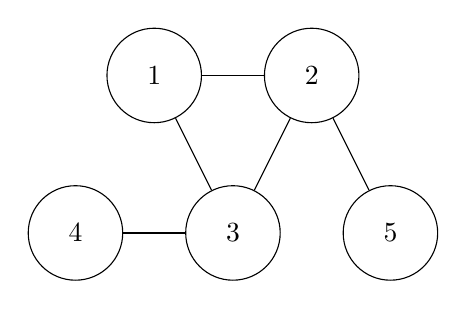
\begin{tikzpicture}[scale=1]
    % ノードの定義
    \node[circle, draw, minimum size=1.2cm] (A) at (0, 0) {1}; 
    \node[circle, draw, minimum size=1.2cm] (B) at (2, 0) {2};
    \node[circle, draw, minimum size=1.2cm] (C) at (1, -2) {3};
    \node[circle, draw, minimum size=1.2cm] (D) at (-1, -2) {4};
    \node[circle, draw, minimum size=1.2cm] (E) at (3, -2) {5};

    % 無向エッジを引く
    \draw (A) -- (B);
    \draw (A) -- (C);
    \draw (B) -- (C);
    \draw (C) -- (D);
    \draw (B) -- (E);

  \end{tikzpicture}
\end{center}
\begin{center}
  無向グラフ
\end{center}
\vspace{0.5cm}

\begin{center}
  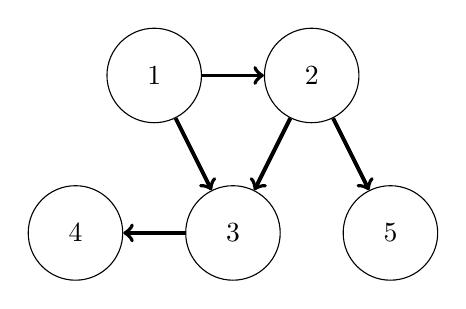
\begin{tikzpicture}[scale=1]
    % ノードの定義
    \node[circle, draw, minimum size=1.2cm] (A) at (0, 0) {1}; 
    \node[circle, draw, minimum size=1.2cm] (B) at (2, 0) {2};
    \node[circle, draw, minimum size=1.2cm] (C) at (1, -2) {3};
    \node[circle, draw, minimum size=1.2cm] (D) at (-1, -2) {4};
    \node[circle, draw, minimum size=1.2cm] (E) at (3, -2) {5};

    % 太い有向エッジを引く
    \draw[->, line width=0.5mm] (A) -- (B);
    \draw[->, line width=0.5mm] (A) -- (C);
    \draw[->, line width=0.5mm] (B) -- (C);
    \draw[->, line width=0.5mm] (C) -- (D);
    \draw[->, line width=0.5mm] (B) -- (E);

  \end{tikzpicture}
\end{center}

\begin{center}
  有向グラフ
\end{center}

\subsection{重み付きグラフ}
重み付きグラフはエッジに重みがついたグラフです。重みはエッジのコストや距離を表します。

\begin{center}
  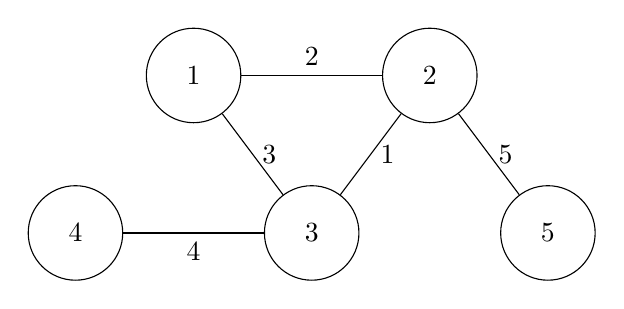
\begin{tikzpicture}[scale=1, auto, node distance=2cm, every loop/.style={}]
    % ノードの定義
    \node[circle, draw, minimum size=1.2cm] (A) at (0, 0) {1}; 
    \node[circle, draw, minimum size=1.2cm] (B) at (3, 0) {2};
    \node[circle, draw, minimum size=1.2cm] (C) at (1.5, -2) {3};
    \node[circle, draw, minimum size=1.2cm] (D) at (-1.5, -2) {4};
    \node[circle, draw, minimum size=1.2cm] (E) at (4.5, -2) {5};

    % エッジと重みを描く
    \draw[-] (A) -- (B) node[midway, above] {2};
    \draw[-] (A) -- (C) node[midway, right] {3};
    \draw[-] (B) -- (C) node[midway, right] {1};
    \draw[-] (C) -- (D) node[midway, below] {4};
    \draw[-] (B) -- (E) node[midway, right] {5};

  \end{tikzpicture}
\end{center}

\subsection{隣接行列と隣接リスト}

隣接行列と隣接リストはグラフを表現するためのデータ構造です。
以下のグラフを例にして、隣接行列と隣接リストを示します。

\begin{center}
  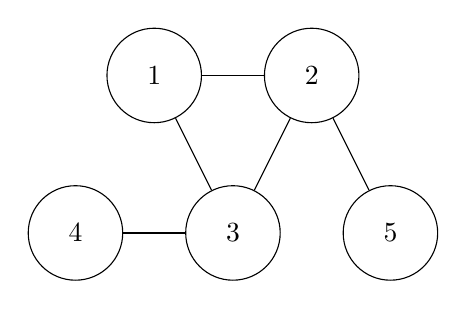
\begin{tikzpicture}[scale=1]
    % ノードの定義
    \node[circle, draw, minimum size=1.2cm] (A) at (0, 0) {1}; 
    \node[circle, draw, minimum size=1.2cm] (B) at (2, 0) {2};
    \node[circle, draw, minimum size=1.2cm] (C) at (1, -2) {3};
    \node[circle, draw, minimum size=1.2cm] (D) at (-1, -2) {4};
    \node[circle, draw, minimum size=1.2cm] (E) at (3, -2) {5};

    % 無向エッジを引く
    \draw (A) -- (B);
    \draw (A) -- (C);
    \draw (B) -- (C);
    \draw (C) -- (D);
    \draw (B) -- (E);

  \end{tikzpicture}
\end{center}
\subsubsection*{隣接行列}

隣接行列はグラフのエッジを行列で表現したものです。$(i, j)$成分が1のとき、ノード$i$とノード$j$がエッジで結ばれていることを表します。下の図では
隣接行列は1-indexedで表現しています。

\[
\begin{pmatrix}
0 & 1 & 1 & 0 & 0 \\
1 & 0 & 1 & 0 & 1 \\
1 & 1 & 0 & 1 & 0 \\
0 & 0 & 1 & 0 & 0 \\
0 & 1 & 0 & 0 & 0 \\
\end{pmatrix}
\]

\subsubsection*{隣接リスト}
隣接リストは各ノードに隣接するノードをリストで表現したものです。

\begin{itemize}
  \item 1: 2, 3
  \item 2: 1, 3, 5
  \item 3: 1, 2, 4
  \item 4: 3
  \item 5: 2
\end{itemize}

\newpage

グラフの基本として、深さ優先探索(DFS)と幅優先探索(BFS)というグラフの探索アルゴリズムを扱います。
\section{幅優先探索(BFS)}
BFSは、後戻りしないように、可能性のあるルートすべてにおいて1ステップずつ行くアルゴリズムです。BFS
の例を見てみましょう。

\vspace{0.5cm}

\begin{center}
  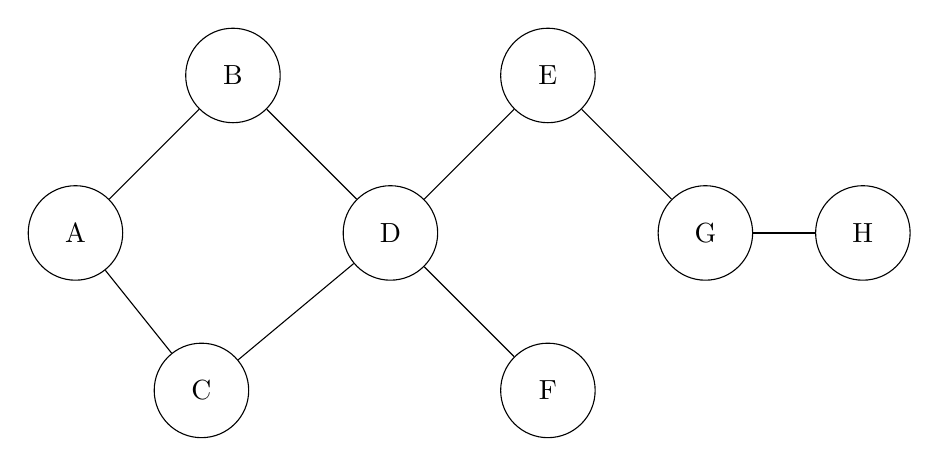
\begin{tikzpicture}
    % ノード
    \node[circle, draw, minimum size=1.2cm] (A) at (-4, 0) {A};
    \node[circle, draw, minimum size=1.2cm] (B) at (-2, 2) {B};
    \node[circle, draw, minimum size=1.2cm] (C) at (-2.4, -2) {C};
    \node[circle, draw, minimum size=1.2cm] (D) at (0, 0) {D};
    \node[circle, draw, minimum size=1.2cm] (E) at (2, 2) {E};
    \node[circle, draw, minimum size=1.2cm] (F) at (2, -2) {F};
    \node[circle, draw, minimum size=1.2cm] (G) at (4, 0) {G};
    \node[circle, draw, minimum size=1.2cm] (H) at (6, 0) {H};

    % エッジ
    \draw (A) -- (B);
    \draw (A) -- (C);
    \draw (C) -- (D);
    \draw (B) -- (D);
    \draw (D) -- (E);
    \draw (D) -- (F);
    \draw (E) -- (G);
    \draw (G) -- (H);
  \end{tikzpicture}
\end{center}
\vspace{0.5cm}

Aからスタートします。

\vspace{0.5cm}

\begin{center}
  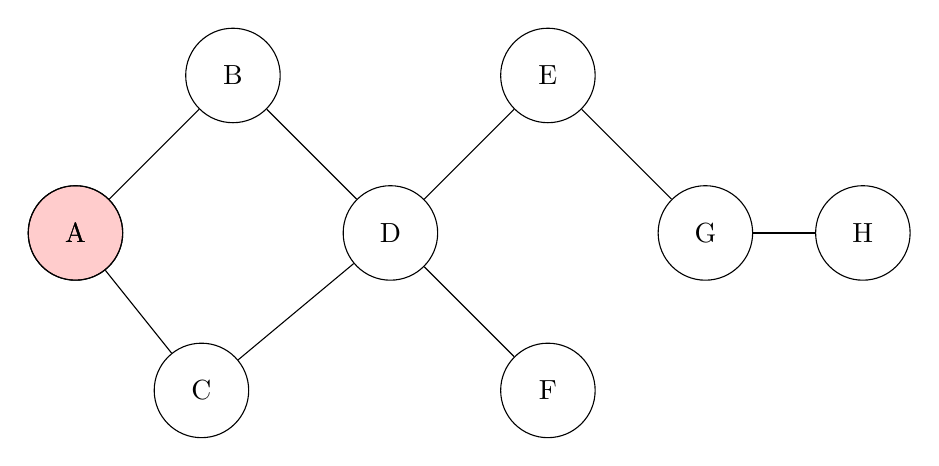
\begin{tikzpicture}
    % 探索済みノードに赤色を塗る
    \node[circle, draw, minimum size=1.2cm, fill=red!20] (A) at (-4, 0) {A};

    % ノード
    \node[circle, draw, minimum size=1.2cm] (A) at (-4, 0) {A};
    \node[circle, draw, minimum size=1.2cm] (B) at (-2, 2) {B};
    \node[circle, draw, minimum size=1.2cm] (C) at (-2.4, -2) {C};
    \node[circle, draw, minimum size=1.2cm] (D) at (0, 0) {D};
    \node[circle, draw, minimum size=1.2cm] (E) at (2, 2) {E};
    \node[circle, draw, minimum size=1.2cm] (F) at (2, -2) {F};
    \node[circle, draw, minimum size=1.2cm] (G) at (4, 0) {G};
    \node[circle, draw, minimum size=1.2cm] (H) at (6, 0) {H};

    % エッジ
    \draw (A) -- (B);
    \draw (A) -- (C);
    \draw (C) -- (D);
    \draw (B) -- (D);
    \draw (D) -- (E);
    \draw (D) -- (F);
    \draw (E) -- (G);
    \draw (G) -- (H);
  \end{tikzpicture}
\end{center}

次にAと繋がっているノードBとCを探索します。

\vspace{0.5cm}

\begin{center}
  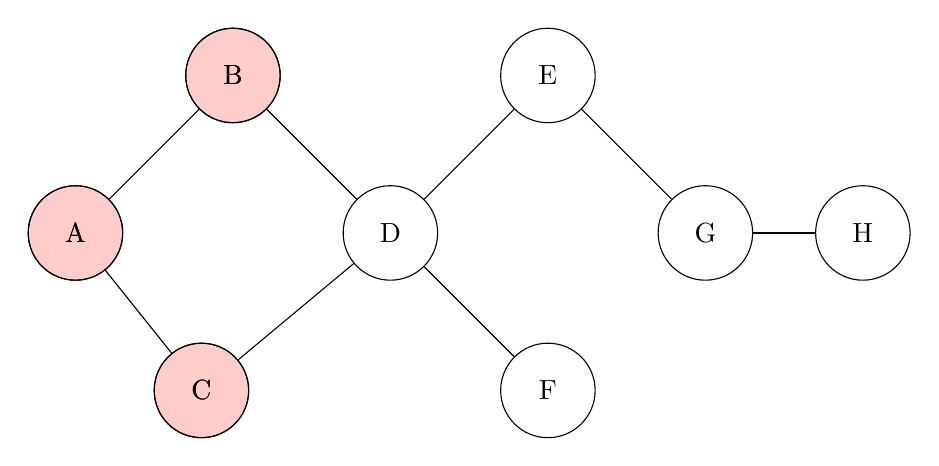
\begin{tikzpicture}
    % 探索済みノードに赤色を塗る
    \node[circle, draw, minimum size=1.2cm, fill=red!20] (A) at (-4, 0) {A};
    \node[circle, draw, minimum size=1.2cm, fill=red!20] (B) at (-2, 2) {B};
    \node[circle, draw, minimum size=1.2cm, fill=red!20] (C) at (-2.4, -2) {C};

    % ノード
    \node[circle, draw, minimum size=1.2cm] (A) at (-4, 0) {A};
    \node[circle, draw, minimum size=1.2cm] (B) at (-2, 2) {B};
    \node[circle, draw, minimum size=1.2cm] (C) at (-2.4, -2) {C};
    \node[circle, draw, minimum size=1.2cm] (D) at (0, 0) {D};
    \node[circle, draw, minimum size=1.2cm] (E) at (2, 2) {E};
    \node[circle, draw, minimum size=1.2cm] (F) at (2, -2) {F};
    \node[circle, draw, minimum size=1.2cm] (G) at (4, 0) {G};
    \node[circle, draw, minimum size=1.2cm] (H) at (6, 0) {H};

    % エッジ
    \draw (A) -- (B);
    \draw (A) -- (C);
    \draw (C) -- (D);
    \draw (B) -- (D);
    \draw (D) -- (E);
    \draw (D) -- (F);
    \draw (E) -- (G);
    \draw (G) -- (H);
  \end{tikzpicture}
\end{center}
\vspace{0.5cm}

Aの探索が終わったので、次にBとCの探索を行います。今回はBから探索します。BとCは同じ深さにあるので、
どちらから探索しても問題ありません。BにはDが繋がっているので、Dを探索します。Cから
探索を始めようとすると、すでにDはすでに探索済みなので、探索を行いません。

\begin{center}
  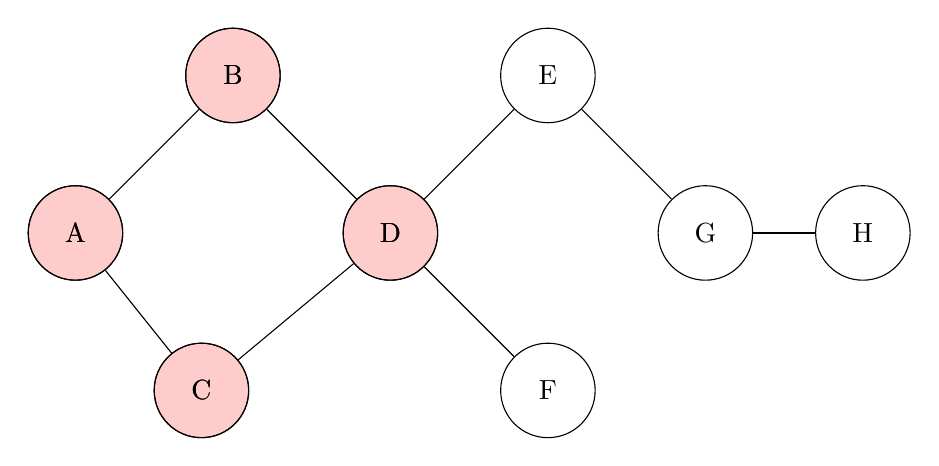
\begin{tikzpicture}
    % 探索済みノードに赤色を塗る
    \node[circle, draw, minimum size=1.2cm, fill=red!20] (A) at (-4, 0) {A};
    \node[circle, draw, minimum size=1.2cm, fill=red!20] (B) at (-2, 2) {B};
    \node[circle, draw, minimum size=1.2cm, fill=red!20] (C) at (-2.4, -2) {C};
    \node[circle, draw, minimum size=1.2cm, fill=red!20] (D) at (0, 0) {D};

    % ノード
    \node[circle, draw, minimum size=1.2cm] (A) at (-4, 0) {A};
    \node[circle, draw, minimum size=1.2cm] (B) at (-2, 2) {B};
    \node[circle, draw, minimum size=1.2cm] (C) at (-2.4, -2) {C};
    \node[circle, draw, minimum size=1.2cm] (D) at (0, 0) {D};
    \node[circle, draw, minimum size=1.2cm] (E) at (2, 2) {E};
    \node[circle, draw, minimum size=1.2cm] (F) at (2, -2) {F};
    \node[circle, draw, minimum size=1.2cm] (G) at (4, 0) {G};
    \node[circle, draw, minimum size=1.2cm] (H) at (6, 0) {H};

    % エッジ
    \draw (A) -- (B);
    \draw (A) -- (C);
    \draw (C) -- (D);
    \draw (B) -- (D);
    \draw (D) -- (E);
    \draw (D) -- (F);
    \draw (E) -- (G);
    \draw (G) -- (H);
  \end{tikzpicture}
\end{center}
\vspace{0.5cm}

次にDから探索を行います。DにはEとFが繋がっているので、EとFを探索します。

\vspace{0.5cm}
\begin{center}
  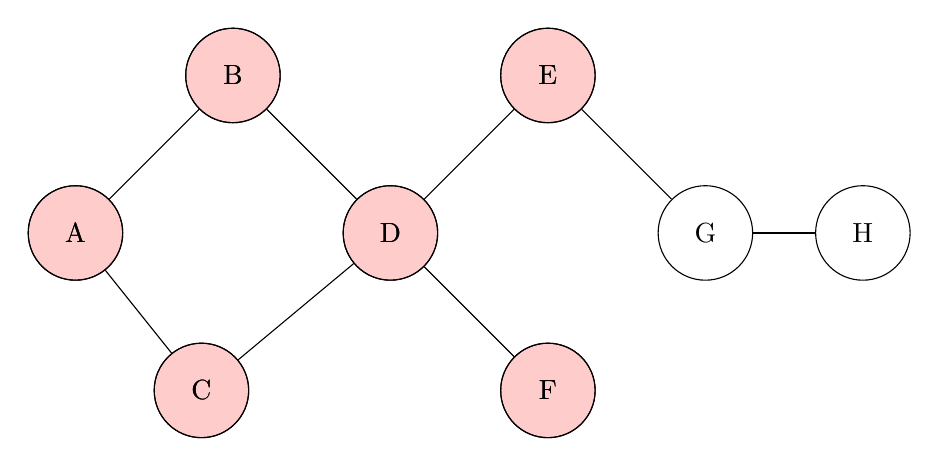
\begin{tikzpicture}
    % 探索済みノードに赤色を塗る
    \node[circle, draw, minimum size=1.2cm, fill=red!20] (A) at (-4, 0) {A};
    \node[circle, draw, minimum size=1.2cm, fill=red!20] (B) at (-2, 2) {B};
    \node[circle, draw, minimum size=1.2cm, fill=red!20] (C) at (-2.4, -2) {C};
    \node[circle, draw, minimum size=1.2cm, fill=red!20] (D) at (0, 0) {D};
    \node[circle, draw, minimum size=1.2cm, fill=red!20] (E) at (2, 2) {E};
    \node[circle, draw, minimum size=1.2cm, fill=red!20] (F) at (2, -2) {F};

    % ノード
    \node[circle, draw, minimum size=1.2cm] (A) at (-4, 0) {A};
    \node[circle, draw, minimum size=1.2cm] (B) at (-2, 2) {B};
    \node[circle, draw, minimum size=1.2cm] (C) at (-2.4, -2) {C};
    \node[circle, draw, minimum size=1.2cm] (D) at (0, 0) {D};
    \node[circle, draw, minimum size=1.2cm] (E) at (2, 2) {E};
    \node[circle, draw, minimum size=1.2cm] (F) at (2, -2) {F};
    \node[circle, draw, minimum size=1.2cm] (G) at (4, 0) {G};
    \node[circle, draw, minimum size=1.2cm] (H) at (6, 0) {H};

    % エッジ
    \draw (A) -- (B);
    \draw (A) -- (C);
    \draw (C) -- (D);
    \draw (B) -- (D);
    \draw (D) -- (E);
    \draw (D) -- (F);
    \draw (E) -- (G);
    \draw (G) -- (H);
  \end{tikzpicture}
\end{center}
\vspace{0.5cm}

最後にGとHを探索します。

\begin{center}
  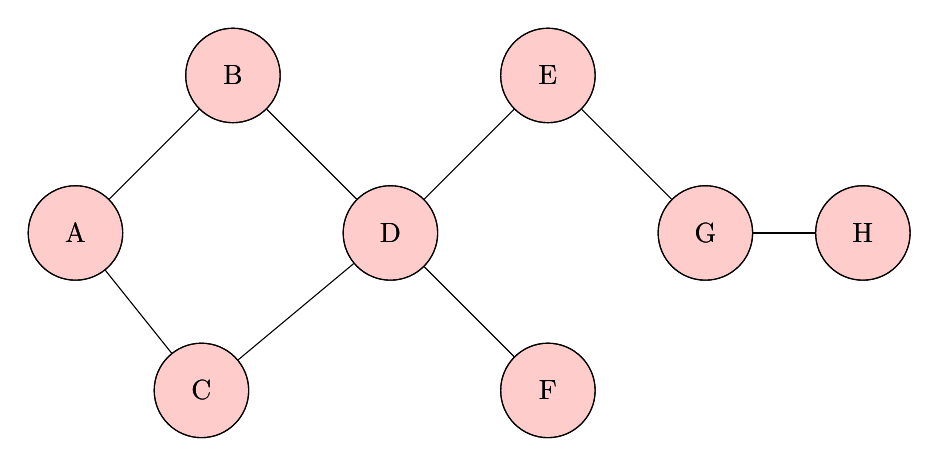
\begin{tikzpicture}
    % 探索済みノードに赤色を塗る
    \node[circle, draw, minimum size=1.2cm, fill=red!20] (A) at (-4, 0) {A};
    \node[circle, draw, minimum size=1.2cm, fill=red!20] (B) at (-2, 2) {B};
    \node[circle, draw, minimum size=1.2cm, fill=red!20] (C) at (-2.4, -2) {C};
    \node[circle, draw, minimum size=1.2cm, fill=red!20] (D) at (0, 0) {D};
    \node[circle, draw, minimum size=1.2cm, fill=red!20] (E) at (2, 2) {E};
    \node[circle, draw, minimum size=1.2cm, fill=red!20] (F) at (2, -2) {F};
    \node[circle, draw, minimum size=1.2cm, fill=red!20] (G) at (4, 0) {G};
    \node[circle, draw, minimum size=1.2cm, fill=red!20] (H) at (6, 0) {H};

    % ノード
    \node[circle, draw, minimum size=1.2cm] (A) at (-4, 0) {A};
    \node[circle, draw, minimum size=1.2cm] (B) at (-2, 2) {B};
    \node[circle, draw, minimum size=1.2cm] (C) at (-2.4, -2) {C};
    \node[circle, draw, minimum size=1.2cm] (D) at (0, 0) {D};
    \node[circle, draw, minimum size=1.2cm] (E) at (2, 2) {E};
    \node[circle, draw, minimum size=1.2cm] (F) at (2, -2) {F};
    \node[circle, draw, minimum size=1.2cm] (G) at (4, 0) {G};
    \node[circle, draw, minimum size=1.2cm] (H) at (6, 0) {H};

    % エッジ
    \draw (A) -- (B);
    \draw (A) -- (C);
    \draw (C) -- (D);
    \draw (B) -- (D);
    \draw (D) -- (E);
    \draw (D) -- (F);
    \draw (E) -- (G);
    \draw (G) -- (H);
  \end{tikzpicture}
\end{center}
\vspace{0.5cm}

これでグラフの探索が終了しました。BFSはスタート地点からの最短距離を求めることができます。

\subsection{BFSの実装}
BFSの実装はキューを用いて行います。実装のポイントは以下の通りです。

\begin{itemize}
  \item キューを用いて、次に探索するノードを管理する
  \item 探索済みのノードを管理するために、配列を用いる
\end{itemize}

隣接リストでも隣接行列でも実装できますが、隣接リストの方が実装が簡単です。また0-indexedで実装している
ことに注意してください。

\begin{lstlisting}[caption=深さ優先探索ヒープの実装, label=bfs, frame=TRBL, label={bfs}]
from collections import deque

  def bfs(graph: list[list[int]], start: int) -> list[bool]:
      visited = [False] * len(graph)
      todo = deque()
      
      # スタート地点で初期化
      todo.append(start)
      
      while todo:
          node = todo.popleft()
          visited[node] = True
          
          for next_node in graph[node]:
              if not visited[next_node]:
                  todo.append(next_node)
                  
      return visited
\end{lstlisting}

\newpage

\section{深さ優先探索(DFS)}
DFSは、スタート地点から次のノードに進み、進んだノードに繋がっているノードを行けなくなるまで探索するアルゴリズムです。
先ほどのグラフを例にして、DFSの探索を行います。

最初はAから探索を行います。

\vspace{0.5cm}

\begin{center}
  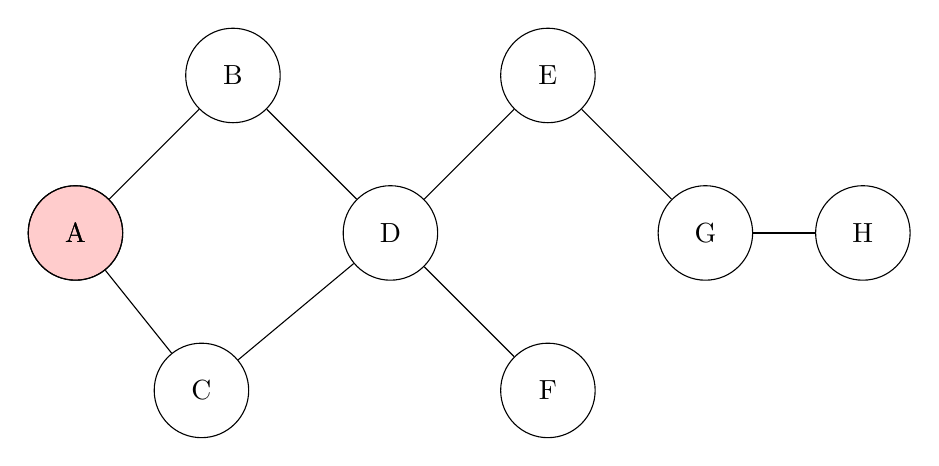
\begin{tikzpicture}
    % 探索済みノードに赤色を塗る
    \node[circle, draw, minimum size=1.2cm, fill=red!20] (A) at (-4, 0) {A};
    % ノード
    \node[circle, draw, minimum size=1.2cm] (A) at (-4, 0) {A};
    \node[circle, draw, minimum size=1.2cm] (B) at (-2, 2) {B};
    \node[circle, draw, minimum size=1.2cm] (C) at (-2.4, -2) {C};
    \node[circle, draw, minimum size=1.2cm] (D) at (0, 0) {D};
    \node[circle, draw, minimum size=1.2cm] (E) at (2, 2) {E};
    \node[circle, draw, minimum size=1.2cm] (F) at (2, -2) {F};
    \node[circle, draw, minimum size=1.2cm] (G) at (4, 0) {G};
    \node[circle, draw, minimum size=1.2cm] (H) at (6, 0) {H};

    % エッジ
    \draw (A) -- (B);
    \draw (A) -- (C);
    \draw (C) -- (D);
    \draw (B) -- (D);
    \draw (D) -- (E);
    \draw (D) -- (F);
    \draw (E) -- (G);
    \draw (G) -- (H);
  \end{tikzpicture}
\end{center}

次にAと繋がっているノードBを探索します。

\vspace{0.5cm}

\begin{center}
  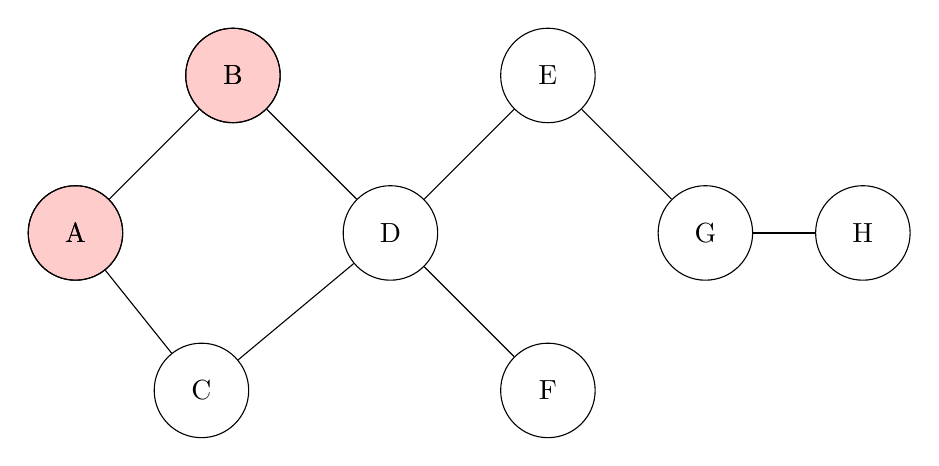
\begin{tikzpicture}
    % 探索済みノードに赤色を塗る
    \node[circle, draw, minimum size=1.2cm, fill=red!20] (A) at (-4, 0) {A};
    \node[circle, draw, minimum size=1.2cm, fill=red!20] (B) at (-2, 2) {B};
    % ノード
    \node[circle, draw, minimum size=1.2cm] (A) at (-4, 0) {A};
    \node[circle, draw, minimum size=1.2cm] (B) at (-2, 2) {B};
    \node[circle, draw, minimum size=1.2cm] (C) at (-2.4, -2) {C};
    \node[circle, draw, minimum size=1.2cm] (D) at (0, 0) {D};
    \node[circle, draw, minimum size=1.2cm] (E) at (2, 2) {E};
    \node[circle, draw, minimum size=1.2cm] (F) at (2, -2) {F};
    \node[circle, draw, minimum size=1.2cm] (G) at (4, 0) {G};
    \node[circle, draw, minimum size=1.2cm] (H) at (6, 0) {H};

    % エッジ
    \draw (A) -- (B);
    \draw (A) -- (C);
    \draw (C) -- (D);
    \draw (B) -- (D);
    \draw (D) -- (E);
    \draw (D) -- (F);
    \draw (E) -- (G);
    \draw (G) -- (H);
  \end{tikzpicture}
\end{center}

\vspace{0.5cm}

BFSではCを次に探索しますが、DFSではBに繋がっているDを探索します。

\vspace{0.5cm}

\begin{center}
  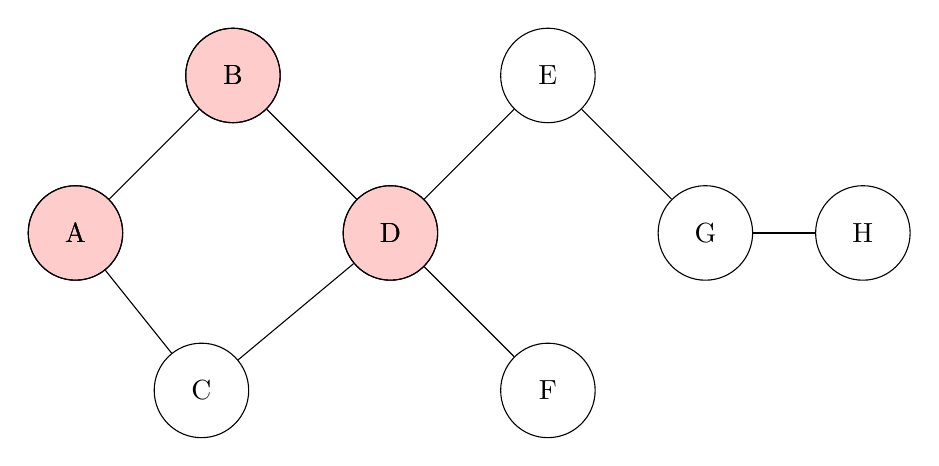
\begin{tikzpicture}
    % 探索済みノードに赤色を塗る
    \node[circle, draw, minimum size=1.2cm, fill=red!20] (A) at (-4, 0) {A};
    \node[circle, draw, minimum size=1.2cm, fill=red!20] (B) at (-2, 2) {B};
    \node[circle, draw, minimum size=1.2cm, fill=red!20] (D) at (0, 0) {D};
    % ノード
    \node[circle, draw, minimum size=1.2cm] (A) at (-4, 0) {A};
    \node[circle, draw, minimum size=1.2cm] (B) at (-2, 2) {B};
    \node[circle, draw, minimum size=1.2cm] (C) at (-2.4, -2) {C};
    \node[circle, draw, minimum size=1.2cm] (D) at (0, 0) {D};
    \node[circle, draw, minimum size=1.2cm] (E) at (2, 2) {E};
    \node[circle, draw, minimum size=1.2cm] (F) at (2, -2) {F};
    \node[circle, draw, minimum size=1.2cm] (G) at (4, 0) {G};
    \node[circle, draw, minimum size=1.2cm] (H) at (6, 0) {H};

    % エッジ
    \draw (A) -- (B);
    \draw (A) -- (C);
    \draw (C) -- (D);
    \draw (B) -- (D);
    \draw (D) -- (E);
    \draw (D) -- (F);
    \draw (E) -- (G);
    \draw (G) -- (H);
  \end{tikzpicture}
\end{center}

\vspace{0.5cm}

次にDに繋がっているEを探索します。

\begin{center}
  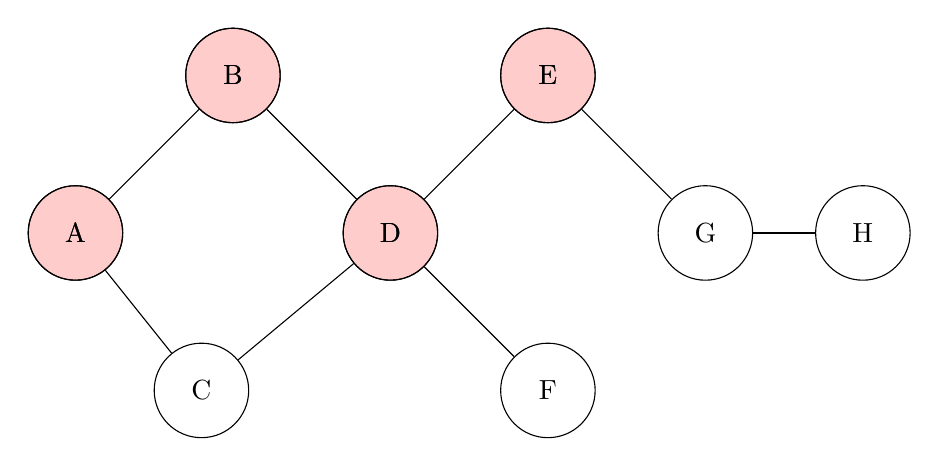
\begin{tikzpicture}
    % 探索済みノードに赤色を塗る
    \node[circle, draw, minimum size=1.2cm, fill=red!20] (A) at (-4, 0) {A};
    \node[circle, draw, minimum size=1.2cm, fill=red!20] (B) at (-2, 2) {B};
    \node[circle, draw, minimum size=1.2cm, fill=red!20] (D) at (0, 0) {D};
    \node[circle, draw, minimum size=1.2cm, fill=red!20] (E) at (2, 2) {E};
    % ノード
    \node[circle, draw, minimum size=1.2cm] (A) at (-4, 0) {A};
    \node[circle, draw, minimum size=1.2cm] (B) at (-2, 2) {B};
    \node[circle, draw, minimum size=1.2cm] (C) at (-2.4, -2) {C};
    \node[circle, draw, minimum size=1.2cm] (D) at (0, 0) {D};
    \node[circle, draw, minimum size=1.2cm] (E) at (2, 2) {E};
    \node[circle, draw, minimum size=1.2cm] (F) at (2, -2) {F};
    \node[circle, draw, minimum size=1.2cm] (G) at (4, 0) {G};
    \node[circle, draw, minimum size=1.2cm] (H) at (6, 0) {H};

    % エッジ
    \draw (A) -- (B);
    \draw (A) -- (C);
    \draw (C) -- (D);
    \draw (B) -- (D);
    \draw (D) -- (E);
    \draw (D) -- (F);
    \draw (E) -- (G);
    \draw (G) -- (H);
  \end{tikzpicture}
\end{center}

これ以上ノードがないノードHまで探索していきます。

\begin{center}
  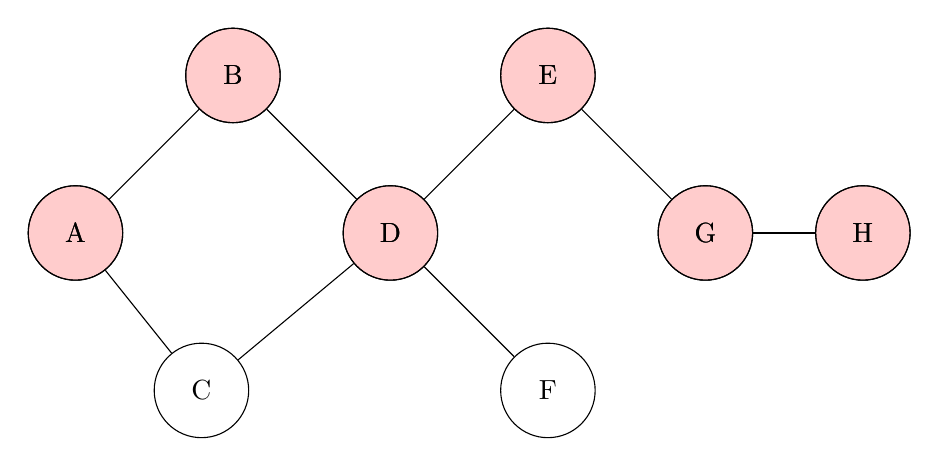
\begin{tikzpicture}
    % 探索済みノードに赤色を塗る
    \node[circle, draw, minimum size=1.2cm, fill=red!20] (A) at (-4, 0) {A};
    \node[circle, draw, minimum size=1.2cm, fill=red!20] (B) at (-2, 2) {B};
    \node[circle, draw, minimum size=1.2cm, fill=red!20] (D) at (0, 0) {D};
    \node[circle, draw, minimum size=1.2cm, fill=red!20] (E) at (2, 2) {E};
    \node[circle, draw, minimum size=1.2cm, fill=red!20] (G) at (4, 0) {G};
    \node[circle, draw, minimum size=1.2cm, fill=red!20] (H) at (6, 0) {H};
    % ノード
    \node[circle, draw, minimum size=1.2cm] (A) at (-4, 0) {A};
    \node[circle, draw, minimum size=1.2cm] (B) at (-2, 2) {B};
    \node[circle, draw, minimum size=1.2cm] (C) at (-2.4, -2) {C};
    \node[circle, draw, minimum size=1.2cm] (D) at (0, 0) {D};
    \node[circle, draw, minimum size=1.2cm] (E) at (2, 2) {E};
    \node[circle, draw, minimum size=1.2cm] (F) at (2, -2) {F};
    \node[circle, draw, minimum size=1.2cm] (G) at (4, 0) {G};
    \node[circle, draw, minimum size=1.2cm] (H) at (6, 0) {H};

    % エッジ
    \draw (A) -- (B);
    \draw (A) -- (C);
    \draw (C) -- (D);
    \draw (B) -- (D);
    \draw (D) -- (E);
    \draw (D) -- (F);
    \draw (E) -- (G);
    \draw (G) -- (H);
  \end{tikzpicture}
\end{center}

\vspace{0.5cm}
移動する余地の残っているFを探索します。

\vspace{0.5cm}

\begin{center}
  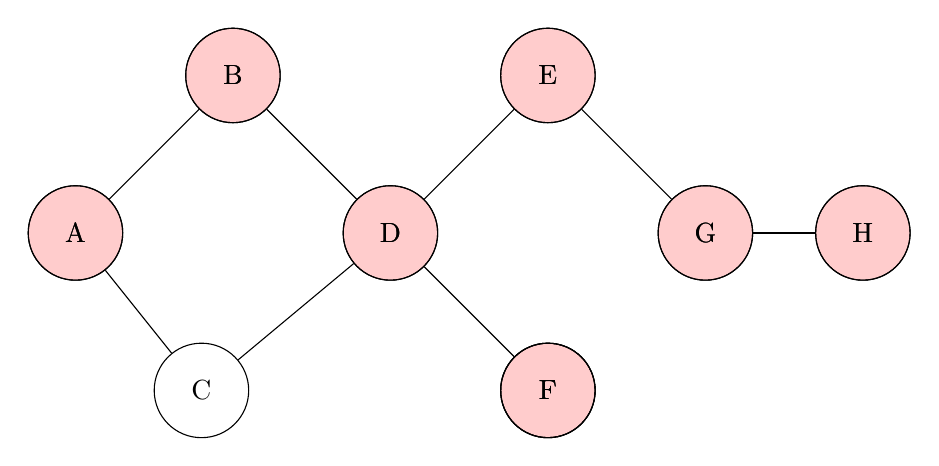
\begin{tikzpicture}
    % 探索済みノードに赤色を塗る
    \node[circle, draw, minimum size=1.2cm, fill=red!20] (A) at (-4, 0) {A};
    \node[circle, draw, minimum size=1.2cm, fill=red!20] (B) at (-2, 2) {B};
    \node[circle, draw, minimum size=1.2cm, fill=red!20] (D) at (0, 0) {D};
    \node[circle, draw, minimum size=1.2cm, fill=red!20] (E) at (2, 2) {E};
    \node[circle, draw, minimum size=1.2cm, fill=red!20] (G) at (4, 0) {G};
    \node[circle, draw, minimum size=1.2cm, fill=red!20] (F) at (2, -2) {F};
    \node[circle, draw, minimum size=1.2cm, fill=red!20] (H) at (6, 0) {H};
    \node[circle, draw, minimum size=1.2cm] (F) at (2, -2) {F};
    % ノード
    \node[circle, draw, minimum size=1.2cm] (A) at (-4, 0) {A};
    \node[circle, draw, minimum size=1.2cm] (B) at (-2, 2) {B};
    \node[circle, draw, minimum size=1.2cm] (C) at (-2.4, -2) {C};
    \node[circle, draw, minimum size=1.2cm] (D) at (0, 0) {D};
    \node[circle, draw, minimum size=1.2cm] (E) at (2, 2) {E};
    \node[circle, draw, minimum size=1.2cm] (F) at (2, -2) {F};
    \node[circle, draw, minimum size=1.2cm] (G) at (4, 0) {G};
    \node[circle, draw, minimum size=1.2cm] (H) at (6, 0) {H};

    % エッジ
    \draw (A) -- (B);
    \draw (A) -- (C);
    \draw (C) -- (D);
    \draw (B) -- (D);
    \draw (D) -- (E);
    \draw (D) -- (F);
    \draw (E) -- (G);
    \draw (G) -- (H);
  \end{tikzpicture}
\end{center}

\vspace{0.5cm}

最後にまだ探索できるAに繋がっているCの探索を行います。

\vspace{0.5cm}

\begin{center}
  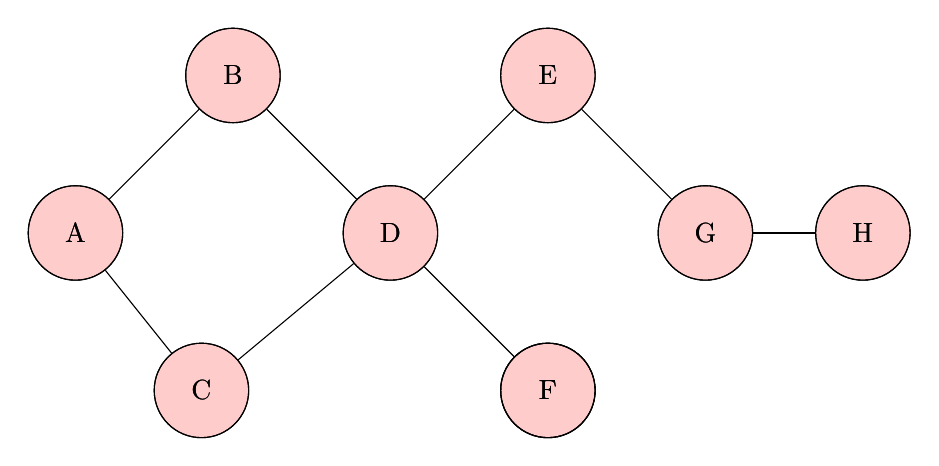
\begin{tikzpicture}
    % 探索済みノードに赤色を塗る
    \node[circle, draw, minimum size=1.2cm, fill=red!20] (A) at (-4, 0) {A};
    \node[circle, draw, minimum size=1.2cm, fill=red!20] (B) at (-2, 2) {B};
    \node[circle, draw, minimum size=1.2cm, fill=red!20] (D) at (0, 0) {D};
    \node[circle, draw, minimum size=1.2cm, fill=red!20] (E) at (2, 2) {E};
    \node[circle, draw, minimum size=1.2cm, fill=red!20] (G) at (4, 0) {G};
    \node[circle, draw, minimum size=1.2cm, fill=red!20] (F) at (2, -2) {F};
    \node[circle, draw, minimum size=1.2cm, fill=red!20] (H) at (6, 0) {H};
    \node[circle, draw, minimum size=1.2cm] (F) at (2, -2) {F};
    \node[circle, draw, minimum size=1.2cm, fill=red!20] (C) at (-2.4, -2) {C};
    % ノード
    \node[circle, draw, minimum size=1.2cm] (A) at (-4, 0) {A};
    \node[circle, draw, minimum size=1.2cm] (B) at (-2, 2) {B};
    \node[circle, draw, minimum size=1.2cm] (C) at (-2.4, -2) {C};
    \node[circle, draw, minimum size=1.2cm] (D) at (0, 0) {D};
    \node[circle, draw, minimum size=1.2cm] (E) at (2, 2) {E};
    \node[circle, draw, minimum size=1.2cm] (F) at (2, -2) {F};
    \node[circle, draw, minimum size=1.2cm] (G) at (4, 0) {G};
    \node[circle, draw, minimum size=1.2cm] (H) at (6, 0) {H};

    % エッジ
    \draw (A) -- (B);
    \draw (A) -- (C);
    \draw (C) -- (D);
    \draw (B) -- (D);
    \draw (D) -- (E);
    \draw (D) -- (F);
    \draw (E) -- (G);
    \draw (G) -- (H);
  \end{tikzpicture}
\end{center}

\vspace{0.5cm}

これでグラフの探索が終了しました。DFSは猪突猛進な探索方法で、BFSとは異なり、最短経路を求めることができません。

\subsection{DFSの実装(スタック)}
DFSの実装はスタックを用いて行います。実装のポイントは以下の通りです。

\begin{itemize}
  \item スタックを用いて、次に探索するノードを管理する
  \item 探索済みのノードを管理するために、配列を用いる
\end{itemize}

隣接リストでも隣接行列でも実装できますが、隣接リストの方が実装が簡単です。また0-indexedで実装している
ことに注意してください。DFSとの違いは、キューをスタックに変えるだけです。

\begin{lstlisting}[caption=深さ優先探索ヒープの実装, label=dfs, frame=TRBL, label={dfs}]
  from collections import deque

  def dfs(graph: list[list[int]], start: int) -> list[bool]:
      visited = [False] * len(graph)
      todo = deque()
      
      # スタート地点で初期化
      todo.append(start)
      
      while todo:
          node = todo.pop()
          visited[node] = True
          
          for next_node in graph[node]:
              if not visited[next_node]:
                  todo.append(next_node)
                  
      return visited
\end{lstlisting}
\subsection{DFSの実装(再帰)}
DFSは再帰を用いて実装することもできます。再帰を用いると、スタックを用いた実装よりも簡潔に実装することができます。

\begin{lstlisting}[caption=深さ優先探索再帰の実装, label=dfs_recursive, frame=TRBL, label={dfs_recursive}]
def dfs(graph: list[list[int]], start: int, visited: list[bool]) -> list[bool]:   
    visited[start] = True
    for next_node in graph[start]:
        if visited[next_node]:
            continue
        else:
            dfs(graph, next_node, visited)
    
    return visited
\end{lstlisting}

\newpage
\section{BFSとDFSを用いた問題}
BFSとDFSは実装はシンプルですが、応用先は広いです。以下にいくつかの問題を紹介します。
\subsection{最短経路問題}
\subsection{オイラーツアー}
\subsection{LCA}
\subsection{橋の検出}

\newpage
\section{最短経路問題}
DFSを用いた最短経路は上で紹介しましたが、今回はより効率的な最短経路問題の解法を紹介します。

\subsection{ダイクストラ法}
\subsection{ベルマンフォード法}
\subsection{SPFA(Shortest Path Faster Algorithm)}
\subsection{ワーシャルフロイド法}

\newpage

\section{最小全域木}
\newpage

\section{トポロジカルソート}

\newpage

\section{最大流問題}


\end{document}
\end{document}